\documentclass[tikz]{standalone}

\usepackage{pgfplots}
\pgfplotsset{ytick style={draw=none}}
\pgfplotsset{xtick style={draw=none}}
\usepackage{helvet}
\usepackage[eulergreek]{sansmath}
\pgfplotsset{
  tick label style = {font=\sansmath\sffamily\small},
  every axis label = {font=\sansmath\sffamily\small},
  legend style = {font=\sansmath\sffamily\small},
  label style = {font=\sansmath\sffamily\small},
  nodes near coords style={font=\sansmath\sffamily\footnotesize},
  title style={font=\sansmath\sffamily\normalsize}
}

\definecolor{GREEN}{RGB}{169,209,142}
\definecolor{ROSE}{RGB}{243,177,131}
\definecolor{BLUE}{RGB}{157,194,230}

\begin{document}

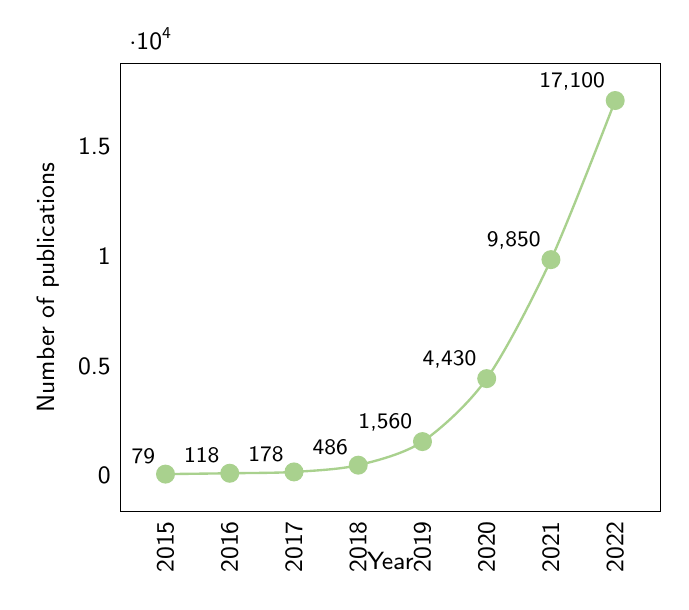
\begin{tikzpicture}
\begin{axis}[
    scatter,
    legend pos=south east,
    xlabel={Year},
    xtick=data,
    %title={Number of Google Scholar GNN publications},
    ylabel={Number of publications},
    x label style={at={(axis description cs:0.5,-0.07)},anchor=north},
    title style={at={(axis description cs:0.5,1.15)},anchor=north},
    xticklabels={2015,2016,2017,2018,2019,2020,2021,2022},
    x tick label style={rotate=90, /pgf/number format/.cd, set thousands separator={}},
    nodes near coords,
    nodes near coords style={color=black},
    nodes near coords align={above left},
]
\addplot+[smooth, mark=*, mark options={scale=1.5,fill=GREEN, color=GREEN}, draw=GREEN, line width=.03cm] 
    coordinates {
    (0,79) (1, 118) (2, 178) (3, 486) (4, 1560) (5, 4430) (6, 9850) (7, 17100)
    };
\end{axis}
\end{tikzpicture}

\end{document}